%! Author = tumbar
%! Date = 1/31/21

% Preamble
\documentclass[11pt]{article}

% Packages
\usepackage{amsmath}
\usepackage[pdfborder={0 0 0},plainpages=false,pdfpagelabels]{hyperref}
\usepackage{tikz}
\usepackage{circuitikzgit}
\usepackage{xifthen}
\usetikzlibrary{circuits.logic.IEC,calc}
\def\code#1{\texttt{#1}}

\makeatletter
\newcommand\currentcoordinate{\the\tikz@lastxsaved,\the\tikz@lastysaved}

% Document
\begin{document}
	\ctikzset{logic ports=ieee}

    \section*{Lab 4 prelab}
    Andrei Tumbar

    \begin{figure}[h!]
        \centering
        %! suppress = Ellipsis
        \begin{circuitikz}[american, ]

            \tikzset{mux16/.style={muxdemux,muxdemux def={Lh=16, NL=16, Rh=14, NB=1, w=3, square pins=0}}}
            \tikzset{aluop/.style={dipchip, num pins=4, hide numbers, no topmark, external pins width=0}}

            % Define the inputs
            \draw (-2.5,1) coordinate(A);
            \draw (-2.5,.5) coordinate(B);
            \draw (A) to[multiwire] ++(-0.5,0) node [anchor=east]{A};
            \draw (B) to[multiwire=N] ++(-0.5,0) node [anchor=east]{B};

            % Generate each of the ALU operations are a dipchip
            \def\Ops{
                % Right side
                OR/0/4,
                AND/0/2,
                XOR/0/0,
                SLL/0/-2,
                SRL/0/-4,
                SRA/0/-6};

            \def\OpPinLength{0.2};
            \def\OpPins{
                % output pin on the right
                out/4/1/left,
                % input pins on the left
                a/1/-1/right,
                b/2/-1/right};

            \foreach \name/\x/\y in \Ops {
                \node [aluop](\name) at (\x,\y) {\name};

                % Generate the input and output pins
                \foreach \subname/\pin/\direction/\labelside in \OpPins {
                    \draw (\name.bpin \pin) -- ++(\OpPinLength*\direction,0) coordinate(\name_\subname);
                    \node [\labelside, font=\tiny] at (\name.bpin \pin) {\subname};
                }
            }

            % Draw the 16 select mux (4 input mux)
            \node [mux16, anchor=lpin 8](ALU) at (4,0){MUX};

            % Label the left pins on the mux in their decimal values
            \foreach \i [evaluate=\i as \pin using int(\i+1)] in {0,...,15} {
                \node [right, font=\tiny] at (ALU.blpin \pin) {\i};
            }

            % Label the select on the mux
            \node [above, font=\tiny] at (ALU.bbpin 1) {op};
            
            

            % 3 tuple (CHIP_NAME, BINARY_OPERATOR, MUX_PIN)
            \def\aluinputs{
                 OR/1000/8/0,
                AND/1010/10/0,
                XOR/1011/11/0,
                SLL/1100/12/0,
                SRL/1101/13/-1,
                SRA/1110/14/-3};

            \def\ALUpinspace{-0.2} % spacing between output lins
            \def\ALUpinoffset{-0.8} % offset from the ALU lpin

            \def\OpAoffset{-0.2}
            \def\OpBoffset{-0.6}

            % Pins that are not bound to an operation
            \def\undefinedpins{0,1,2,3,7,9,15}

            % Draw connections from the ALU mux pin to the operators output
            % Also add a label for the binary equivalent value
            \foreach \name/\binlabel/\pin/\spacescale [count=\xi, evaluate=\pin as \pinreal using int(\pin+1)] in \aluinputs {
                \draw (ALU.lpin \pinreal) -- ++(\spacescale*\ALUpinspace + \xi*\ALUpinspace + \ALUpinoffset,0)
                    to [short, -] (\currentcoordinate |- \name_out) % go to y-coord for output
                    node[label={[shift={(0,0.3)}, font=\footnotesize] left:\binlabel}] {} % label the wire
                    to[short, -] (\name_out); % connect to the x-coord

                % Connect the input pins on each operator
                \draw (\name_a) -- ++(\OpAoffset,0) to [short, *-*] (\currentcoordinate |- A) -- (A);
                \draw (\name_b) -- ++(\OpBoffset,0) to [short, *-*] (\currentcoordinate |- B) -- (B);
            }

            % Create a ground to handle undefined select pins
            \draw (ALU.south west) ++(-0.4, -0.2) node[sground](g){};

            % Connect the undefined pins to ground
            \foreach /\pin [count=\xi, evaluate=\pin as \pinreal using int(\pin+1)] in \undefinedpins {
                \draw (ALU.lpin \pinreal) -- (g |- \currentcoordinate) to [short, *-] (g);
            }
            
            % Connect pins from other diagrams
            \draw (ALU.lpin 5) -| ++(-0.4, 3.4) node[label={[font=\footnotesize]right:Adder}] {};
            
            \draw (ALU.lpin 5) ++(-0.4,0) to [short, *-] (\currentcoordinate |- ALU.lpin 6) -- (ALU.lpin 6);
            
            \draw (ALU.lpin 7) -| ++(-0.6, 4.5) node[label={[font=\footnotesize]left:Multiplier}] {}; 
            

            % Connect the OP signal to the mux select
            \draw (ALU.bpin 1) to[multiwire=4] ++(0,-2) node [anchor=north] (OP){OP};

            % Connect the output 'Y' signal to the mux output
            \draw (ALU.rpin 1) to[multiwire=N] ++(2,0) node[anchor=west] (Y){Y};

        \end{circuitikz}
        \caption{Layout of the N-bit ALU with eight operations}
        \label{fig:block}
    \end{figure}
    
    This ALU will expand on the ALU create in Exercise 1. It will support
    three more operations: multiply, add, subtract.
    The addition and subtraction come from the same circuit. 
    
    \pagebreak
    \begin{figure}[htbp]
    	\centering
		\begin{circuitikz}
		
		\def\Adders{
                % Right side
                A0/0,
                A1/1,
                A2/2,
                AN/n};
		
		\foreach \name/\c [count=\xi, evaluate=\xi as \i using int(\xi - 1),
								evaluate=\xi as \ilast using int(\xi - 2)] in \Adders {
			\draw (\i * 3,0) node[dipchip,
				num pins=6,
				hide numbers, no topmark, external pins width=0.0](a\i){$A_\c$};
			
			\node [right, font=\tiny] at (a\i.bpin 1) {$A_\c$};
			\node [right, font=\tiny] at (a\i.bpin 2) {$B_\c$};
			\node [right, font=\tiny] at (a\i.bpin 3) {$C_{in}$};
			\node [left, font=\tiny]  at (a\i.bpin 6) {$S_\c$};
			\node [left, font=\tiny]  at (a\i.bpin 4) {$C_{out}$};
			
			% Connect the C_out to C_in
			\ifthenelse{\NOT 0 = \i \AND \NOT 3 = \i} {
				\draw (a\ilast.bpin 4) -- (a\i.bpin 3);
			}{
				\ifthenelse{3 = \i}{
					\draw (a\ilast.bpin 4) to [short,l=..., -] (a\i.bpin 3);
				}{};
			};
			
			% Wire the first input
			\draw (a\i.bpin 1) -| ++(-0.2, 0.5)
				node[label={[font=\footnotesize]above:$A_\c$}] {};
			
			% Wire the second input to an XOR gate to handle subtraction
			\draw (a\i.bpin 2) -| ++(-0.8, 0.7) node[ieeestd xor
port, rotate=-90, anchor=out, scale=0.6](a\i_xor) {};
			
			\ifthenelse{\NOT 0 = \i}
			{
				\draw (a\i_xor.in 1) -- ++(0, 0.2) to [short, -*]
					(a\ilast_xor.in 1 |- \currentcoordinate);
			}{};
			
			% Wire the second input of the XOR gate
			\draw (a\i_xor.in 2) -- ++(0, 0.5)
				node[label={[font=\footnotesize]above:$B_\c$}] {};
		}
		
		\draw (a0_xor.in 1) |- ++(-1, 0.2) coordinate(alucoordin);
		\draw (a0.bpin 3) -- ++(-1.4, 0) to [short, -*]
			(\currentcoordinate |- alucoordin);
		
		\draw (alucoordin) node[label={[font=\footnotesize]left:\code{ALUControl(0)}}] {};
		
		\end{circuitikz}
	\caption{N-bit ripple-carry adder/subtractor.}
	\label{fig:ripple}
\end{figure}

The output of the adder/subtractor can be found in $S_n$ ports on each full adder. A set LSB on \code{ALUControl} will select subtraction and compute \code{A-B}.
	
	\begin{figure}[htbp]
    	\centering
		\begin{circuitikz}
		
		\draw (0, 2) coordinate (A)
			node[label={[font=\footnotesize]left:A}] {};
		\draw (0, 1) coordinate (B)
			node[label={[font=\footnotesize]left:B}] {};
		\draw (0, 0) coordinate (C)
			node[label={[font=\footnotesize]left:$C_{in}$}] {};
		
		\draw (1.5, 1.5)
			node[ieeestd xor port, scale=0.6](xor1) {};
		\draw (xor1.in 1) -- ++(-0.2, 0) coordinate(xor1_1);
		\draw (xor1.in 2) -- ++(-0.2, 0) coordinate(xor1_2);
		
		\draw (3, 0.5)
			node[ieeestd xor port, scale=0.6](xor2) {};
		\draw (xor2.in 1) -- ++(-0.2, 0) coordinate(xor2_1);
		\draw (xor2.in 2) -- ++(-0.2, 0) coordinate(xor2_2);
		
		\draw (A) -| (xor1_1);
		\draw (B) -| (xor1_2);
		
		\draw (xor1.out) -| (xor2_1);
		\draw (C) -| (xor2_2);
		
		\draw (xor2.out) -- ++(0.3, 0)
			node[label={[font=\footnotesize]right:$S$}] {};
		
		\draw (0, -1) coordinate (Ac)
			node[label={[font=\footnotesize]left:A}] {};
		\draw (0, -2) coordinate (Bc)
			node[label={[font=\footnotesize]left:B}] {};
		\draw (0, -3) coordinate (Cc)
			node[label={[font=\footnotesize]left:$C_{in}$}] {};

		% A(B+C) + BC
		\draw (1, -2)
			node[ieeestd or port, scale=0.6, anchor=in 1](boc) {};
		\draw (1, -3)
			node[ieeestd and port, scale=0.6, anchor=in 1](bc) {};
		
		\draw (Bc) |- (boc.in 1);
		\draw (Cc) to [short, -*] (bc.in 1);
		\draw (bc.in 1) -- (boc.in 2);
		
		\draw (bc.in 2) -- ++(-0.2, 0) to[short, -*] (Bc -| \currentcoordinate);
		
		\draw (boc.out) ++(0.2, 0)
			node[ieeestd and port, scale=0.6, anchor=in 2](aboc) {};
		\draw (boc.out) -- (aboc.in 2);
		\draw (Ac) -| (aboc.in 1);
		
		\draw (aboc.out) ++(0.4, 0)
			node[ieeestd or port, scale=0.6, anchor=in 1](abocbc) {};
		
		\draw (aboc.out) -| (abocbc.in 1);
		\draw (bc.out) -| (abocbc.in 2);
		
		\draw (abocbc.out) -- ++(0.3, 0)
			node[label={[font=\footnotesize]right:$C_{out}$}] {};

		\end{circuitikz}
		\caption{Full-adder circuit diagram}
		\label{fig:FA}
	\end{figure}

	Figure \ref{fig:FA} shows the inner circuit diagram of the full adders used in
	the ripply-carry adders (Figure \ref{fig:ripple}) and the multiplier.
	
	\pagebreak
	
	To multiply numbers $A$ and $B$, a circuit diagram using a grid of full
	adders is shown. A and B are each $N/2$ bits long and the resultant product
	is $N$ bits long.
	
	\begin{figure}[h!]
        \centering
        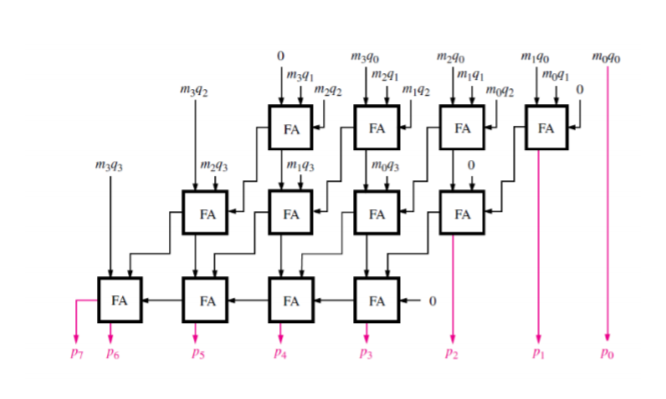
\includegraphics[width=\textwidth]{multiplier}
        \caption{Diagram of a 4-bit unsigned integer multiplier circuit}
        %! suppress = FigureNotReferenced
        \label{fig:demo6}
    \end{figure}

\end{document}

\begin{figure}[htbp]
    	\centering
		\begin{circuitikz}
		\def\RowN1{2};
		\def\ColN1{3};
		
		\foreach \i [count=\xi, evaluate=\xi as \ilast using int(\xi - 1)] in {0,...,\RowN1}
		{
			\foreach \j [count=\xj, evaluate=\xj as \jlast using int(\xj - 1)] in {0,...,\ColN1}
			{
				\draw (1.2*\j - \i * 0.5, -1.5*\i)
					node[qfpchip, hide numbers, scale=0.5]{FA};
			
				\ifthenelse{\NOT \i = 0}
				{
					
				}{};
			};
		};

		\end{circuitikz}
		\caption{N-bit unsigned integer binary multiplier}
		\label{fig:mult}
	\end{figure}